\newcommand{\CLASSINPUTtoptextmargin}{0.75in}
\newcommand{\CLASSINPUTbottomtextmargin}{0.75in}
\newcommand{\CLASSINPUTinnersidemargin}{0.75in}
\newcommand{\CLASSINPUToutersidemargin}{0.75in}
\documentclass[letterpaper,conference,10pt]{ieeetran}
\IEEEoverridecommandlockouts
\overrideIEEEmargins
\pdfoptionpdfminorversion=4
%\usepackage[sc]{mathpazo}
%\linespread{1.02}         % Palatino needs more leading (space between lines)
\usepackage[T1]{fontenc}


\usepackage{multicol}
% Insert hyperlinks in the document
\usepackage{hyperref}
\hypersetup{bookmarksopen,bookmarksnumbered,
pdfpagemode=UseOutlines,
colorlinks=true,
linkcolor=blue,
anchorcolor=blue,
citecolor=blue,
filecolor=blue,
menucolor=blue,
urlcolor=blue
}
\usepackage{amsmath, amssymb, amsfonts, amsthm}
\usepackage{bm}
%\usepackage{subcaption}
\usepackage{flushend}
\usepackage{dirtree}
\usepackage{graphicx}
\usepackage{mathtools}
\usepackage[sort]{natbib}
\usepackage{fixltx2e}

% Labels in IEEE format
\newcommand{\eref}[1]{(\ref{#1})} % Equation
\newcommand{\sref}[1]{Sec. \ref{#1}} % Section
\newcommand{\figref}[1]{Fig.\ref{#1}} % Figure
\newcommand{\tref}[1]{Table \ref{#1}} % Table



% floats
\usepackage[font=footnotesize]{caption} % incompatible with aaai.sty?
%\usepackage[font=footnotesize]{subcaption}
\usepackage{mathabx}
\usepackage{verbatim}
\usepackage{algorithm}
\usepackage{amsmath}
\usepackage[noend]{algpseudocode}


\usepackage{multirow}
\usepackage{booktabs}
\usepackage[dvipsnames]{xcolor}

\setlength{\textfloatsep}{5pt}
\setlength{\intextsep}{5pt}

\newcommand{\ssnote}[1]{{\xxnote{SS}{red}{#1}}}
\newcommand{\scnote}[1]{{\xxnote{SC}{blue}{#1}}}
\newcommand{\cdnote}[1]{{\xxnote{CD}{cyan}{#1}}}
\newcommand{\xxnote}[3]{}
\ifx\hidenotes\undefined
 \usepackage{color}
 \renewcommand{\xxnote}[3]{\color{#2}{#1: #3}}
\fi

\ifCLASSOPTIONcompsoc
  \usepackage[caption=false,font=normalsize,labelfont=sf,textfont=sf]{subfig}
\else
  \usepackage[caption=false,font=footnotesize]{subfig}
\fi

\DeclareMathOperator*{\argmin}{\arg\!\min}

\begin{document}

\title{\vspace{0.20in}\LARGE Title}

\author{Pengju Jin, Siddhartha Srinivasa}
\maketitle 	

\begin{abstract}
Abstract Goes here
\end{abstract}

\IEEEpeerreviewmaketitle

% !TEX root = ../main.tex
\section{Introduction}
\label{sec:intro}
Detection and identification using artificial landmarks, known as fiducial markers, has long been used in augmented reality and computer vision applications. Over the last decade, there has been numerous marker systems, such as ARTags, Apriltags, and Rune Tags, designed to improve detection encoding precision. However, these systems are not robust enough to be used reliability in many robotic applications.

Compared to markerless detection algorithms, these fiducial marker methods are simpler and more consistent. There has been significant effort in improving the detection speed and encoding accuracy. They have yield great results for computer vision tasks that require high detection accuracy like camera calibrations, 3D reconstruction. Furthermore, they have gained popularity in the robotic community for having unique characteristics of high detection rates and numerous encoding schemes. For example, Apriltags are commonly used to test SLAM systems or finding ground truth for objects in manipulation and motion planning tasks as shown in Figure \ref{fig:table_clearing}. 

Despite all the improvements, obtaining accurate pose estimations from these tags remain a challenge. This is especially important for robotic applications because small errors can cause large system failures as the errors propagate and amplify through the system. Currently, these systems yield good results under well conditioned or rendered environments, but this does not translate to ill-conditioned settings. For instances, when Apriltags are used with low resolution camera or harsh lighting conditions, the system often produce poses with tremendous rotational errors as shown in Figure \ref{fig:mismatch}. In fact, we observe that the localization accuracy of this system perform significantly worse at difficult viewing angles or when there are noise in the scene. This is a difficult problem because RGB sensors are sensitive to lighting and current fiducial systems are not designed to take advantage of other sensors commonly available on robots.

We present two main contributions in this paper. First, we conducted an in-depth analysis on the effect of various noises on the pose estimation process. In particular, the noise in RGB images creates a perspective ambiguity problem that makes the pose estimation challenging without additional information. Second, we describe a novel method that takes advantage of the RGBD sensors that are commonly available on most robotic systems to accurately estimate the pose from a single tag under noisy conditions in real time. In the core of the algorithm, we recognize that RGB and depth sensors work optimally under different conditions. Therefore, their strength can be combined meaningfully to improve the localization accuracy robust to illumination. There are few key features to this algorithm: 
\begin{itemize}
\item This method is highly robust to noise in the scene. It can obtain accurate poses suitable for a wide range robotic applications.   
\item It is easily generalizable to most fiducial tags designs.
\item It performs at worse at least as good as using only RGB images.
\item It has very small computation overhead and can be ran in real time. 
\end{itemize}

This paper also presents empirical results demonstrating the the successful performance of the algorithm on captured data from an humanoid robot. Our implementation of the algorithm is based off of the Apriltag detection pipeline and it is integrated with ROS. 

\begin{figure}
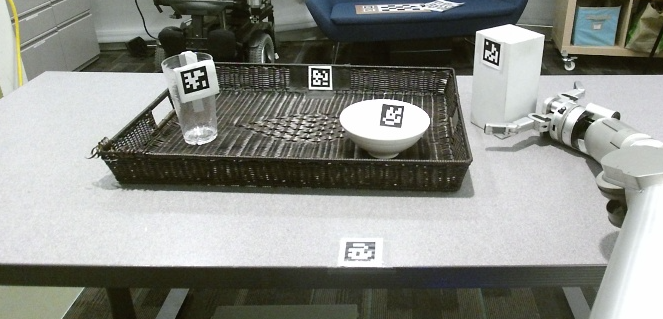
\includegraphics[width=\columnwidth, height=120px]{figs/table_clearing_rgb_small} \\
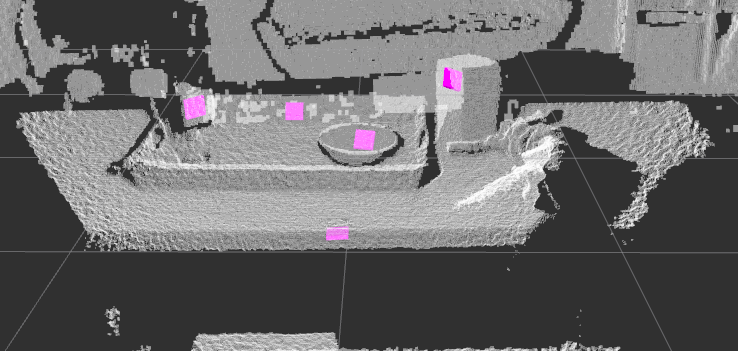
\includegraphics[width=\columnwidth, height=120px]{figs/table_clearing_depth}
\label{fig:table_clearing}
\caption{Apriltag used to localize objects in mainpulation tasks}
\end{figure}

% !TEX root = ../main.tex
\section{Related Work}
\label{sec:related}

Related work here

% !TEX root = ../main.tex
\section{Perceptual Ambiguity}
\label{sec:problem}
In most square fiducial tag detection, the pose is calculated by fitting a quad around the planar tag. The corners are extracted from the tag and the pose is estimated using 3D to 2D point correspondence optimization methods such as Levenberg$-$Marquardt [OpenCV reference] or DLT. This is a specific case of the perspective-n-point problem and it has been well studied in geometry based Computer Vision literatures [][]. In particular, there is a deterministic solution to the perspective-4-point problem. In other words, given the projection of a tag corners, the pose of the tag is unique. In reality, however,  when a small tag is captured in a low resolution camera, the perspective projection becomes almost orthographic. In these cases, a small variance in the corner detection process will yield estimations far from the true pose due to a perceptual ambiguity under projection. 

We will illustrate this effect by using two over lapping cubes in figure 3. The overlapping face of the two cubes are interlaced but rotated by 120 degrees. However, due to perspective projection the squares appears to be on the same plane. Under low camera resolution, the over lapping squares become virtually indistinguishable. The red circular regions are the detected corners under some sensory noise. In these cases, the optimal PnP solution is no longer singular but a bimodal distribution depending on the viewing angle. The result of the 3D to 2D correspondence optimization might return either one of the two solution.
\begin{figure}
\centering
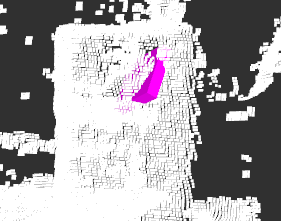
\includegraphics[width=\columnwidth]{figs/mismatch_tag}
\caption{The orientation of Apriltag placed on the object is greatly misaligned with the actual object}
\label{fig:calib}
\end{figure}

\begin{figure}
\centering
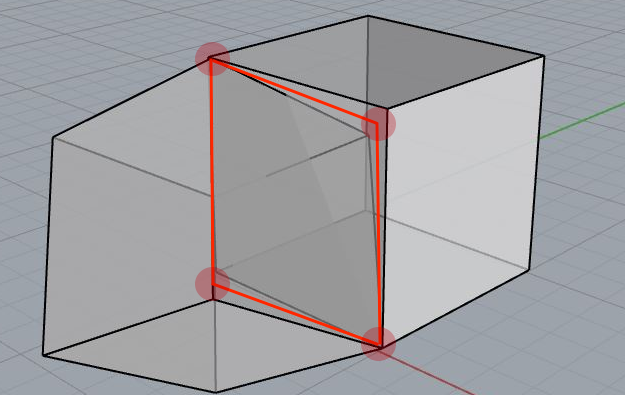
\includegraphics[width=\columnwidth]{figs/perspective_fig}
\caption{Perspective Ambiguity illustrated with overlapping cubes}
\label{fig:calib}
\end{figure}

% !TEX root = ../main.tex
\section{Approach}
\label{sec:approach}
This section describes a method for estimating poses of noisy square fiducial tags using RGBD data. Unlike previous methods, the detected corners of the tag are treated as approximated locations of the true corners. Using the corners, the method implicitly evaluate the depth data and RGB data as two independent observations and fuse them in a meaningful way.

There are three distinct components to this method. First, we find the plane in $SO(3)$ containing the tag using depth data. Secondly, an approximate pose is computed using the depth plane and the corners from tag detection. Finally, the method refines the initial pose using the RGB data. Each component is described in detail in the following subsections and illustrated in Fig. 

\subsection{Depth Plane Fitting}
With a calibrated RGBD sensor, depth and RGB streams are registered to the same frame. The square patch of points in the depth image defined by the $g$ also contains the range information of the tag. Here we take advantage of the planar characteristic of the tag. By fitting a plane over the range data, we can constrain the pose of the tag to be on the plane.

The raw range data retrieved from the Kinect One sensor are usually noisy as illustrated by Figure \ref{fig:depth_data}. Specifically, borders of the tag and some of the dark regions of the tag produce highly unreliable range data. Therefore, we first filter the data by removing points too far from the median before fitting the plane. Nevertheless, the remaining points could have a large variance depending on the lighting condition and the magnitude of the plane rotation. The accuracy of the plane and tag pose is directly affected by the noise level of data. In fact, we want to characterize the uncertainty and weight the initial estimation accordingly during the fusing stage.

In implementation, we used a Bayesian plane fitting algorithm described in [Uncertainty Analysis] which computes the Hessian Normal parameters of a plane through optimizing
\begin{IEEEeqnarray}{c}
\min _{\boldsymbol{\hat{n}}, d} \sum_{j=1}^{N} 
	\frac{(p_j(\boldsymbol{\hat{n}} \cdot \boldsymbol{\hat{m}_j}) -d)^2}
		 {(\boldsymbol{\hat{n}} \cdot \boldsymbol{\hat{m}_j})^2\sigma ^2\{\bar{p}_j \} }
\label{eq:gaussian_noise}
\end{IEEEeqnarray}
The algorithm in the paper assumes a radial Gaussian noise in the range data $p_j$ with the standard deviation modeled by a function in the form
\begin{IEEEeqnarray}{c}
\sigma \{ \bar{p_j} \} = \frac{kd^2}{ \| \boldsymbol{\hat{n}} \cdot \boldsymbol{\hat{m}_j} \| } 
\IEEEeqnarraynumspace
\label{eq:gaussian_noise}
\end{IEEEeqnarray}
where $\boldsymbol{\hat{n}}$ is the local normal to the planar surface of the depth point and $\boldsymbol{\hat{m_j}}$ is the measurement direction for the sensor for point $p_j$. The coefficient $k > 0$ is an estimated value obtained from sensor calibration. In our implementation, we obtained $k$ by simplified the results from [Kinect Noise Model paper]. 

Another important result we used from [] is the covariance matrix for the plane-parameters. The covariance matrix is obtained by taking the \textit{Moore-Penrose generalized inverse} of Hessian matrix computed from the Lagrangian. The covariance characterizes the uncertainty of the plane and defines the refinement regions of the pose later in the pipeline. 

\begin{figure}
\centering
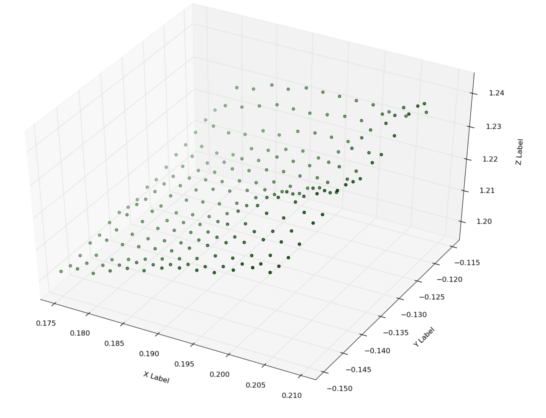
\includegraphics[width=\columnwidth]{figs/depth_plane_fig}
\caption{The depth points of the Apriltag plane. The points are noisy but good for an approximate estimation.}
\label{fig:depth_data}
\end{figure}

\subsection{Initial Pose Estimation}
The pose of the tag can be described as the transformation from tag's frame to the sensory frame of the robot given by $[R, \boldsymbol{t}]$. However, the depth plane $D [ \boldsymbol{\hat{n}}, d]$ alone is insufficient to determine the transformation because it only defines 3 DOF in a 6 DOF space. Furthermore, the center of the tag must align with the center of the plane and thus further constrain 2 DOF. However, there are still infinite number of valid poses rotating about the normal $\boldsymbol{\hat{n}}$. One solution is to constrain the pose by using a corner as an extra point correspondence to solve for the optimal rotation. However, the accuracy of this method largely depends on the depth accuracy of the chosen corner point. 

An alternative is to use all 4 detected corners as 4 pairs of point correspondences for the optimization. We projected the detected corners onto $D [ \boldsymbol{\hat{n}}, d]$ to get the coordinates $p = [p_1, p_2, p_3, p_4]$ in the robot sensory frame. The corner coordinates $q = [q_1, q_2, q_3, q_4]$ in the tag frame can be easily calculated since the tag is a square plane. We define the center of the tag as the origin, the corner coordinates are simply the location of the corners on a Cartesian plane. Given two sets of 3D point correspondences, this can be computed as a rigid body transformation estimation [Reference to SVD 3D rigid body]. Solving for the optimal transformation $[R, \boldsymbol{t}]$ requires minimizing a least squares error objective function given by:
\begin{IEEEeqnarray}{c}
[R, \boldsymbol{t}] = \argmin _{R \in SO(3), \boldsymbol{t}\in \mathbb{R}^3} \sum_{i=1}^{n} w_i \| R \boldsymbol{p_i} + \boldsymbol{t} - \boldsymbol{q_i}\| ^2
\IEEEeqnarraynumspace
\label{eq:rigid_body}
\end{IEEEeqnarray}
There are numerous approaches to solve Eq. \ref{eq:rigid_body}. Since we have very few correspondences and they are assumed to be correct, it can be computed quickly using SVD:
\begin{IEEEeqnarray}{rCl}
& \bar{p} = \frac{1}{N} \sum_{i=1}^{N} p_i \qquad p_{ci} = p_i - \bar{p} \\
& \bar{q} = \frac{1}{N} \sum_{i=1}^{N} q_i \qquad q_{ci} = q_i - \bar{q} 
\end{IEEEeqnarray}
\begin{IEEEeqnarray}{rCl}
p_{c}^{\top}q_c &= U\Sigma V^\top \\
R & = VU^\top\\
\boldsymbol{t} & = \bar{q} - R\bar{p}
\end{IEEEeqnarray}
$R$ and $t$ are the corresponding rotation and translation components of the the transformation. The above approach minimizes the least square error of the transformation and it is robust to small errors in the correspondences. The resulting pose obtained from the range data, although not accurate, is robust to noise and provide a good approximation for the true pose. 

\subsection{Pose Refinement}
\begin{figure}
\centering
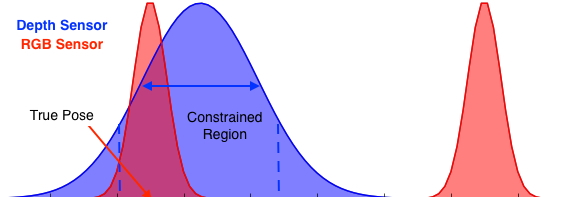
\includegraphics[width=\columnwidth]{figs/optimization_visualization_fig}
\caption{An abstract visualization of the optimization constraints. The blue curve is the initial pose estimation obtained from the depth plane. The red curves are the ambiguous poses from the RGB image. We constrained the region of optimization based on how well we fit the depth plane.}
\label{fig:calib}
\end{figure}
Given the initial pose estimate of the tag and the RGB image, we can refine the pose that minimizes the reprojection error. Given camera model $K$, initial rotation and translation estimates $R_{init}$ and $t_{init}$
\begin{align*}
\hat{y} &= K[(R_{init} + \Delta R)x + (t_{init} + \Delta t)]\\
&\underset{\Delta R, \Delta t}{\mathrm{min}} (y - \hat{y})\\
&\text{subject to:} \\
& |\Delta R| <= \Gamma_R, \; |\Delta t| <= \Gamma_t\\
\end{align*}
The challenge here is to determine the region $\Gamma_R$ and $\Gamma_t$ which the initial pose estimate can be adjusted. If we unbound $\Delta R$ and $\Delta t$ intheon Apriltag detection algorithmson Apriltag detection algorithm the optimization, the solution might converge to a pose optimal for the reprojection error but far away from the true pose due to perceptual ambiguity. On the other hand, if we constrain the optimization too much, the final pose might not be far away from the true pose because of the inaccurate initial estimation. We recognize that the bound of on this optimization is related to the variance of the initial pose estimation. In one extreme, if there is no uncertainty in the depth camera and the range data are perfect, we don't need to further refine the pose of the tag. Similarly, if we don't have any depth information (uncertainty of the initial estimate is infinity), then the best we can do is find the pose solely based on the reprojection error which is the same as solving the unbounded optimization problem. Thererfore, this becomes a constrained optimization problem where the bound on the independent variables of $\Delta R$ and $\Delta t$ is proportional to the covariance of our estimated depth plane parameters. In our implementation, we used the trust-region algorithm to bound the optimization. The scaling threshold parameter is emperically tested to yield the best results for our robot. 

The key insight to our method is that it harness the different strength of RGB and depth information during the pose optimization process. By considering all the points on the tag, the depth data is more robust to noises in the scene. However, range data is inherently inconsistent and the pose is thus imprecise. In contrast, the advantage of RGB image is that the corners can be detected at a sub-pixel precision. It is useful for refinement optimization.  

% !TEX root = ../main.tex
\section{Experimental Results}

The key problem we are trying to resolve is the localization accuracy of Apriltags in noisy situations. Therefore, we want to test the resilience of our algorithm and show that it can obtain reasonable pose estimations under high level of noise. Figure \ref{fig:result_compare} demonstrates an example visualization of the result. We also compare our method against \textit{ar\_track\_alvar}, a popular ARTag detection package that incorporated depth information. Finally, we briefly tested the runtime of the algorithm to show that it remains capable of real time detection. 

In our experiments, we measured the rotational and translation accuracy of the detection algorithms with respect to three different independent variables: viewing angles, distances, and lighting conditions. We placed a standard camera calibration chessboard and an Apriltag of known size on a solid planar board. The Apriltag has a fixed distance from the chessboard. This is used to compute the ground-truth pose for the tag. By using a large chessboard, we can detect the corners to a sub-pixel accuracy and compute accurate ground-truth poses unsusceptible to lighting and sensory noises. 

\subsection{Viewing Angle}

\begin{figure}
\centering
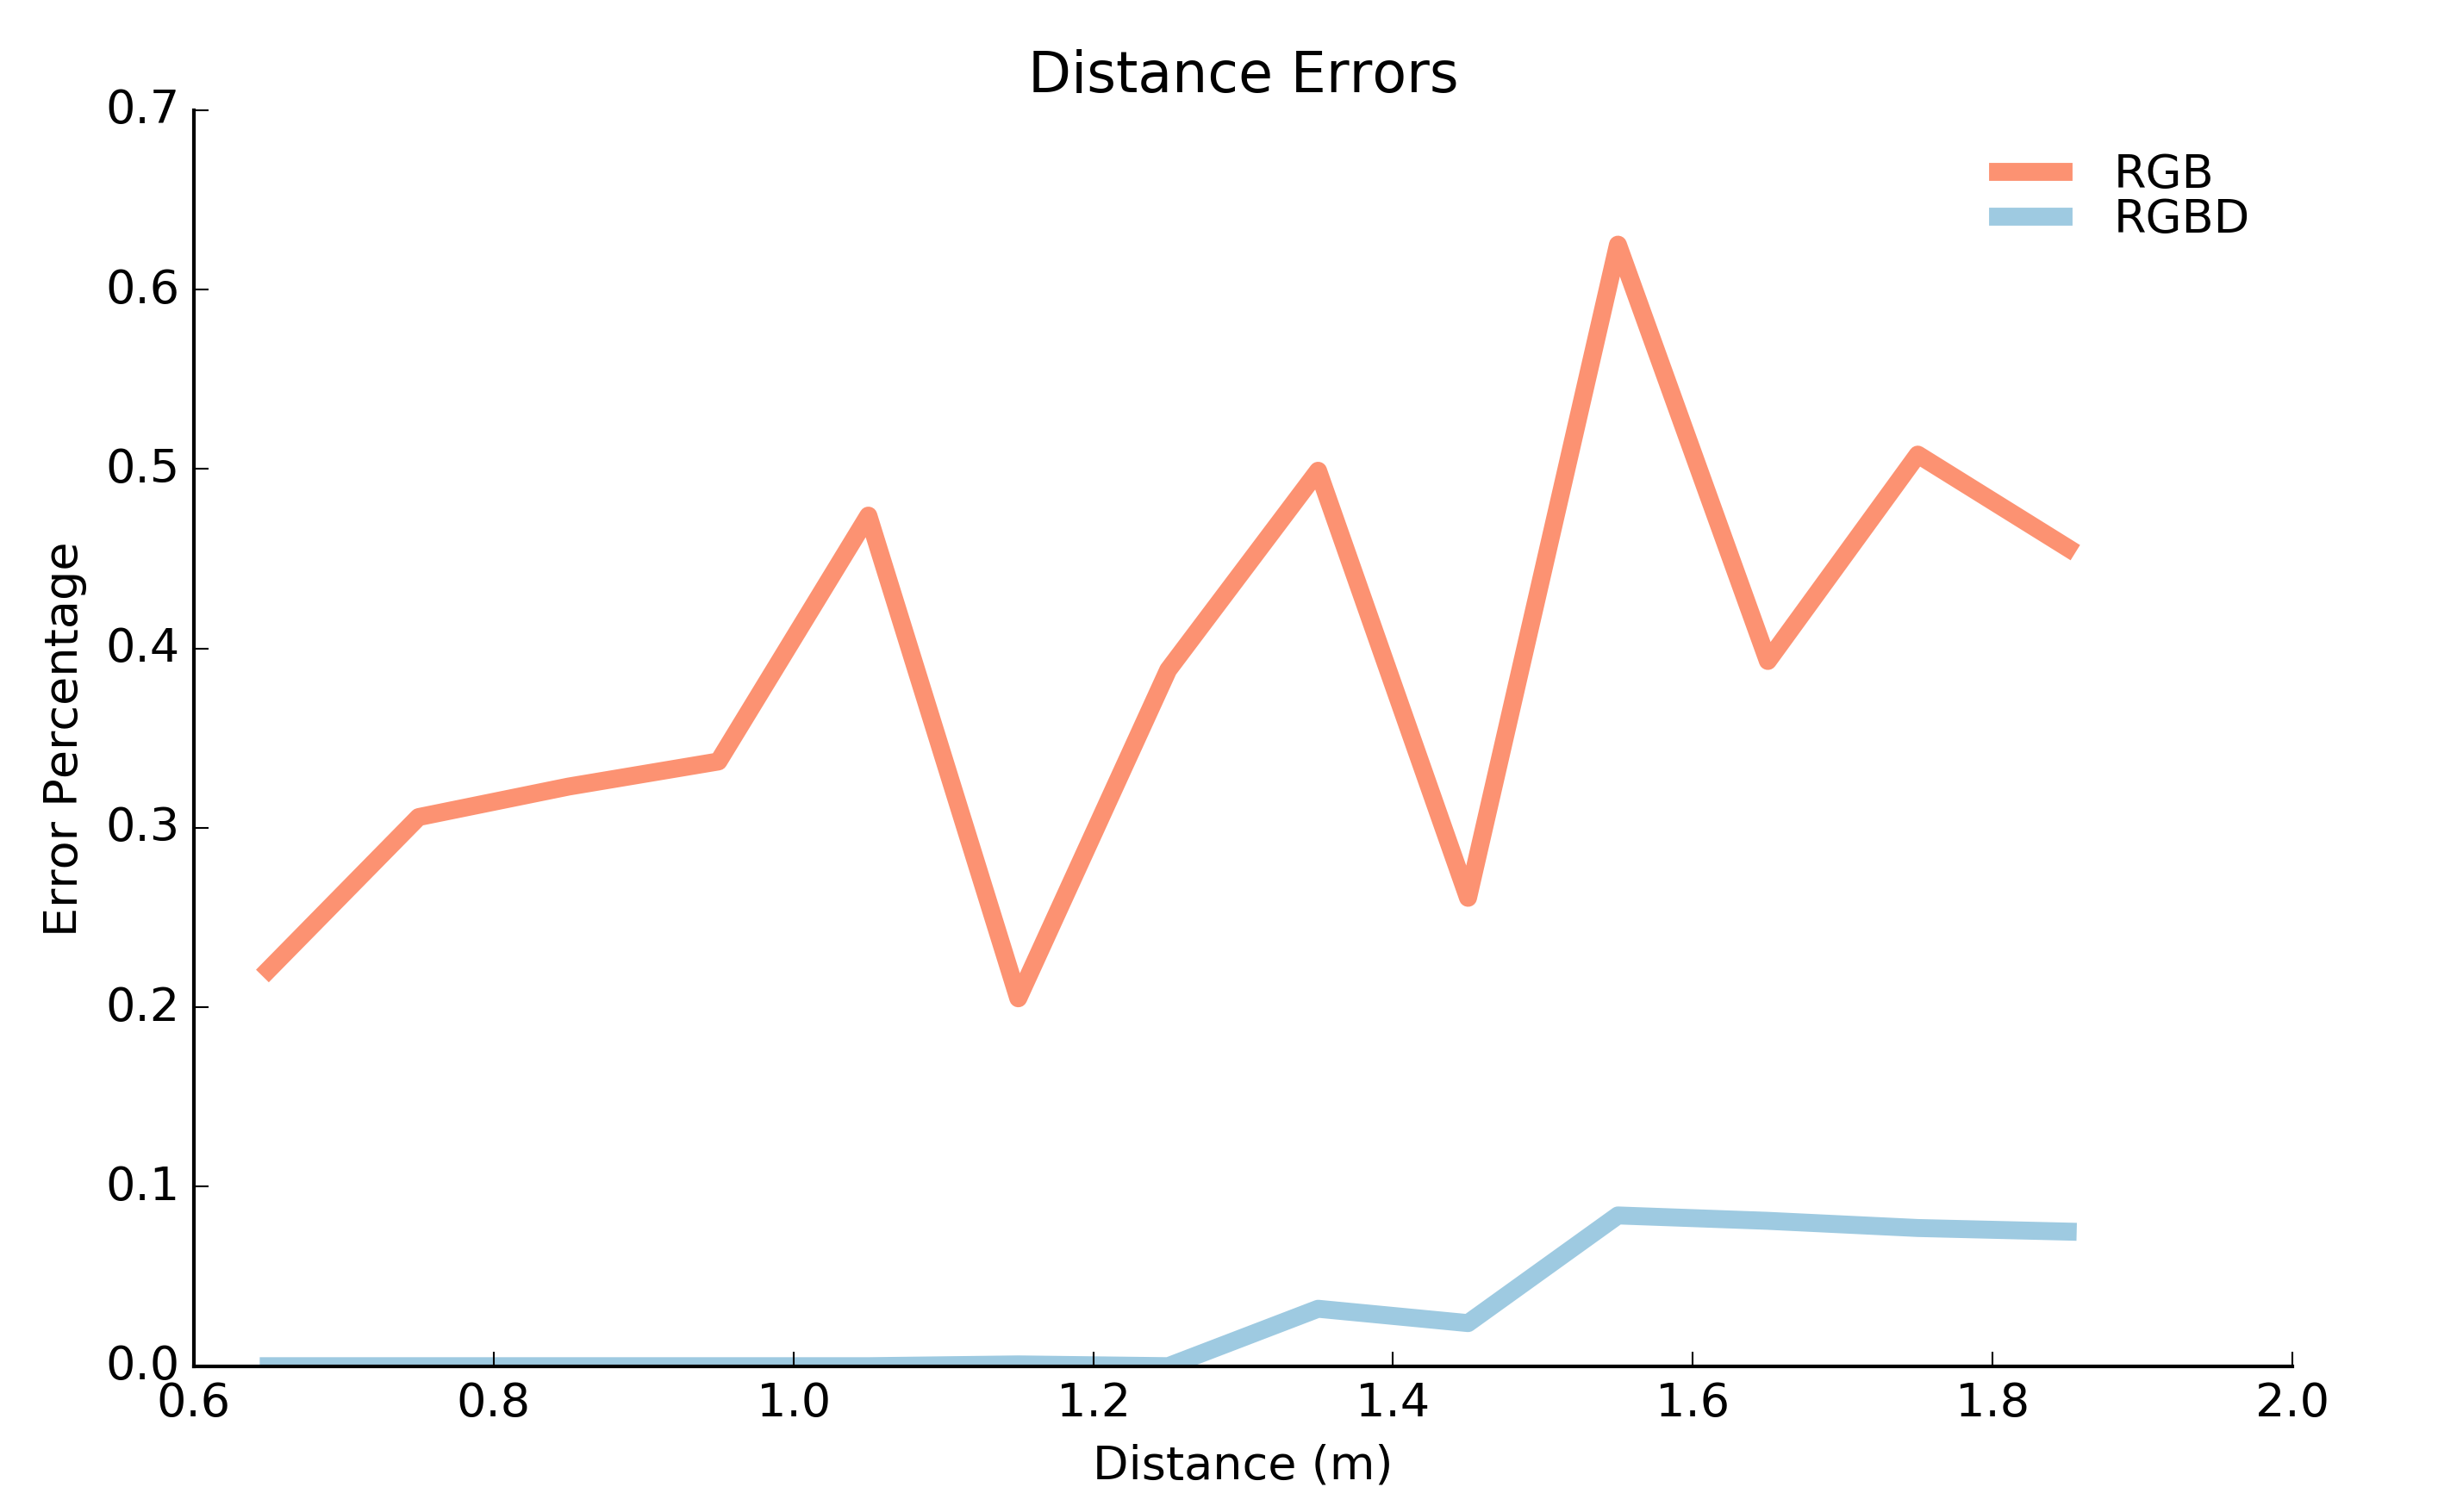
\includegraphics[width=\columnwidth]{figs/distance_fig2}
\caption{Distance vs Error Percentage. Data are captured at a $10$ cm increment from $65$ cm to $185$ cm.}
\label{fig:distance_result}
\end{figure}

Due to the perspective ambiguity effect, the localization accuracy of the Apriltags is heavily affected by the viewing angle of the tag. To characterize the effect, we placed the testing board in front of the robot as shown in \ref{fig:exp_setup}. The testing board is ~$0.65$ meters away from the sensor and rotated it at a increment of 5 degrees from 0 degrees to 60. The angles are measured from the axis parallel to the sensor. This is about the range which the tag can be detected reliably given the camera resolution and the distance. At each angle, we captured the RGB image, depth image, and detection outputs from the Apriltag library. 

For each captured data bundle, we introduced 3 levels of Gaussian noise of $\sigma = 0.2$, $\sigma = 0.5$, $\sigma = 1$  to the RGB image and computed the resulting tag pose. This is repeated for $1000$ trails for each data bundle per noise level and the errors are computed for each trial.  

The empirical result in Figure \ref{fig:bimodal} show a very clear bimodal distribution, as we expected, for the detected poses for a given data bundle over $1000$ trials. In Figure \ref{fig:viewing_result}, we threshold all the poses based on their rotational errors and plotted the percentage of unacceptable poses at each viewing angle. The proposed RGBD fused algorithm vastly outperforms the original algorithm as it has better localization accuracy at all viewing angles and noise levels. 

\subsection{Distance}

%To test the estimation accuracy with respect to distance, we captured the images at different distances away from the camera at a fixed angle. Figure \ref{fig:distance_result} shows the experiment results.
The relationship between the distance and localization accuracy is much more apparent. As the tag moves further away from the sensor, the number of pixels on the tag decreases. The perspective ambiguity effect becomes more apparent when there is only a small patch of pixels on the tag. We show the results of  both RGB and RGBD methods in Figure \ref{fig:distance_result}. During the experiment, it is difficult to keep the viewing angle precisely consistent at each trail. Therefore, the pose error percentage using RGB is not increasing smoothly as they are in the simulation results.

We see a clear increase in error percentage in the proposed method when the tag is far away from the camera. This is contributed both by a smaller tag patch size in the depth image and an increase in noise with the Kinect sensor at a further distance. In these cases, the variance of the depth plane estimation becomes very wide and the algorithm is unable to converge to the correct pose. Nevertheless, our method shows a significant gain in accuracy at every distance.

\begin{figure}
\centering
\subfloat[Dark]{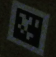
\includegraphics[width=50px, height=50px]{figs/illumination/dark}
\label{fig:dark}}
\subfloat[Dim]{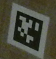
\includegraphics[width=50px, height=50px]{figs/illumination/dim}
\label{fig:dim}}
\subfloat[Normal]{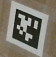
\includegraphics[width=50px, height=50px]{figs/illumination/normal}
\label{fig:normal}}
\subfloat[Bright]{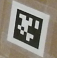
\includegraphics[width=50px, height=50px]{figs/illumination/bright}
\label{fig:bright}}
\caption{Apriltags captured by Kinect V2 under different levels of illumination. The RGB sensor dynamically adjust the exposure time to compensate for low lighting. In \ref{fig:dark}, the image is captured outside of Kinect's adjustable range and the pixels are underexposed. In \ref{fig:dim}, the long exposure time introduced noticeable noise to the image. }
\label{fig:illumination_tag}
\end{figure}

\begin{figure}
\centering
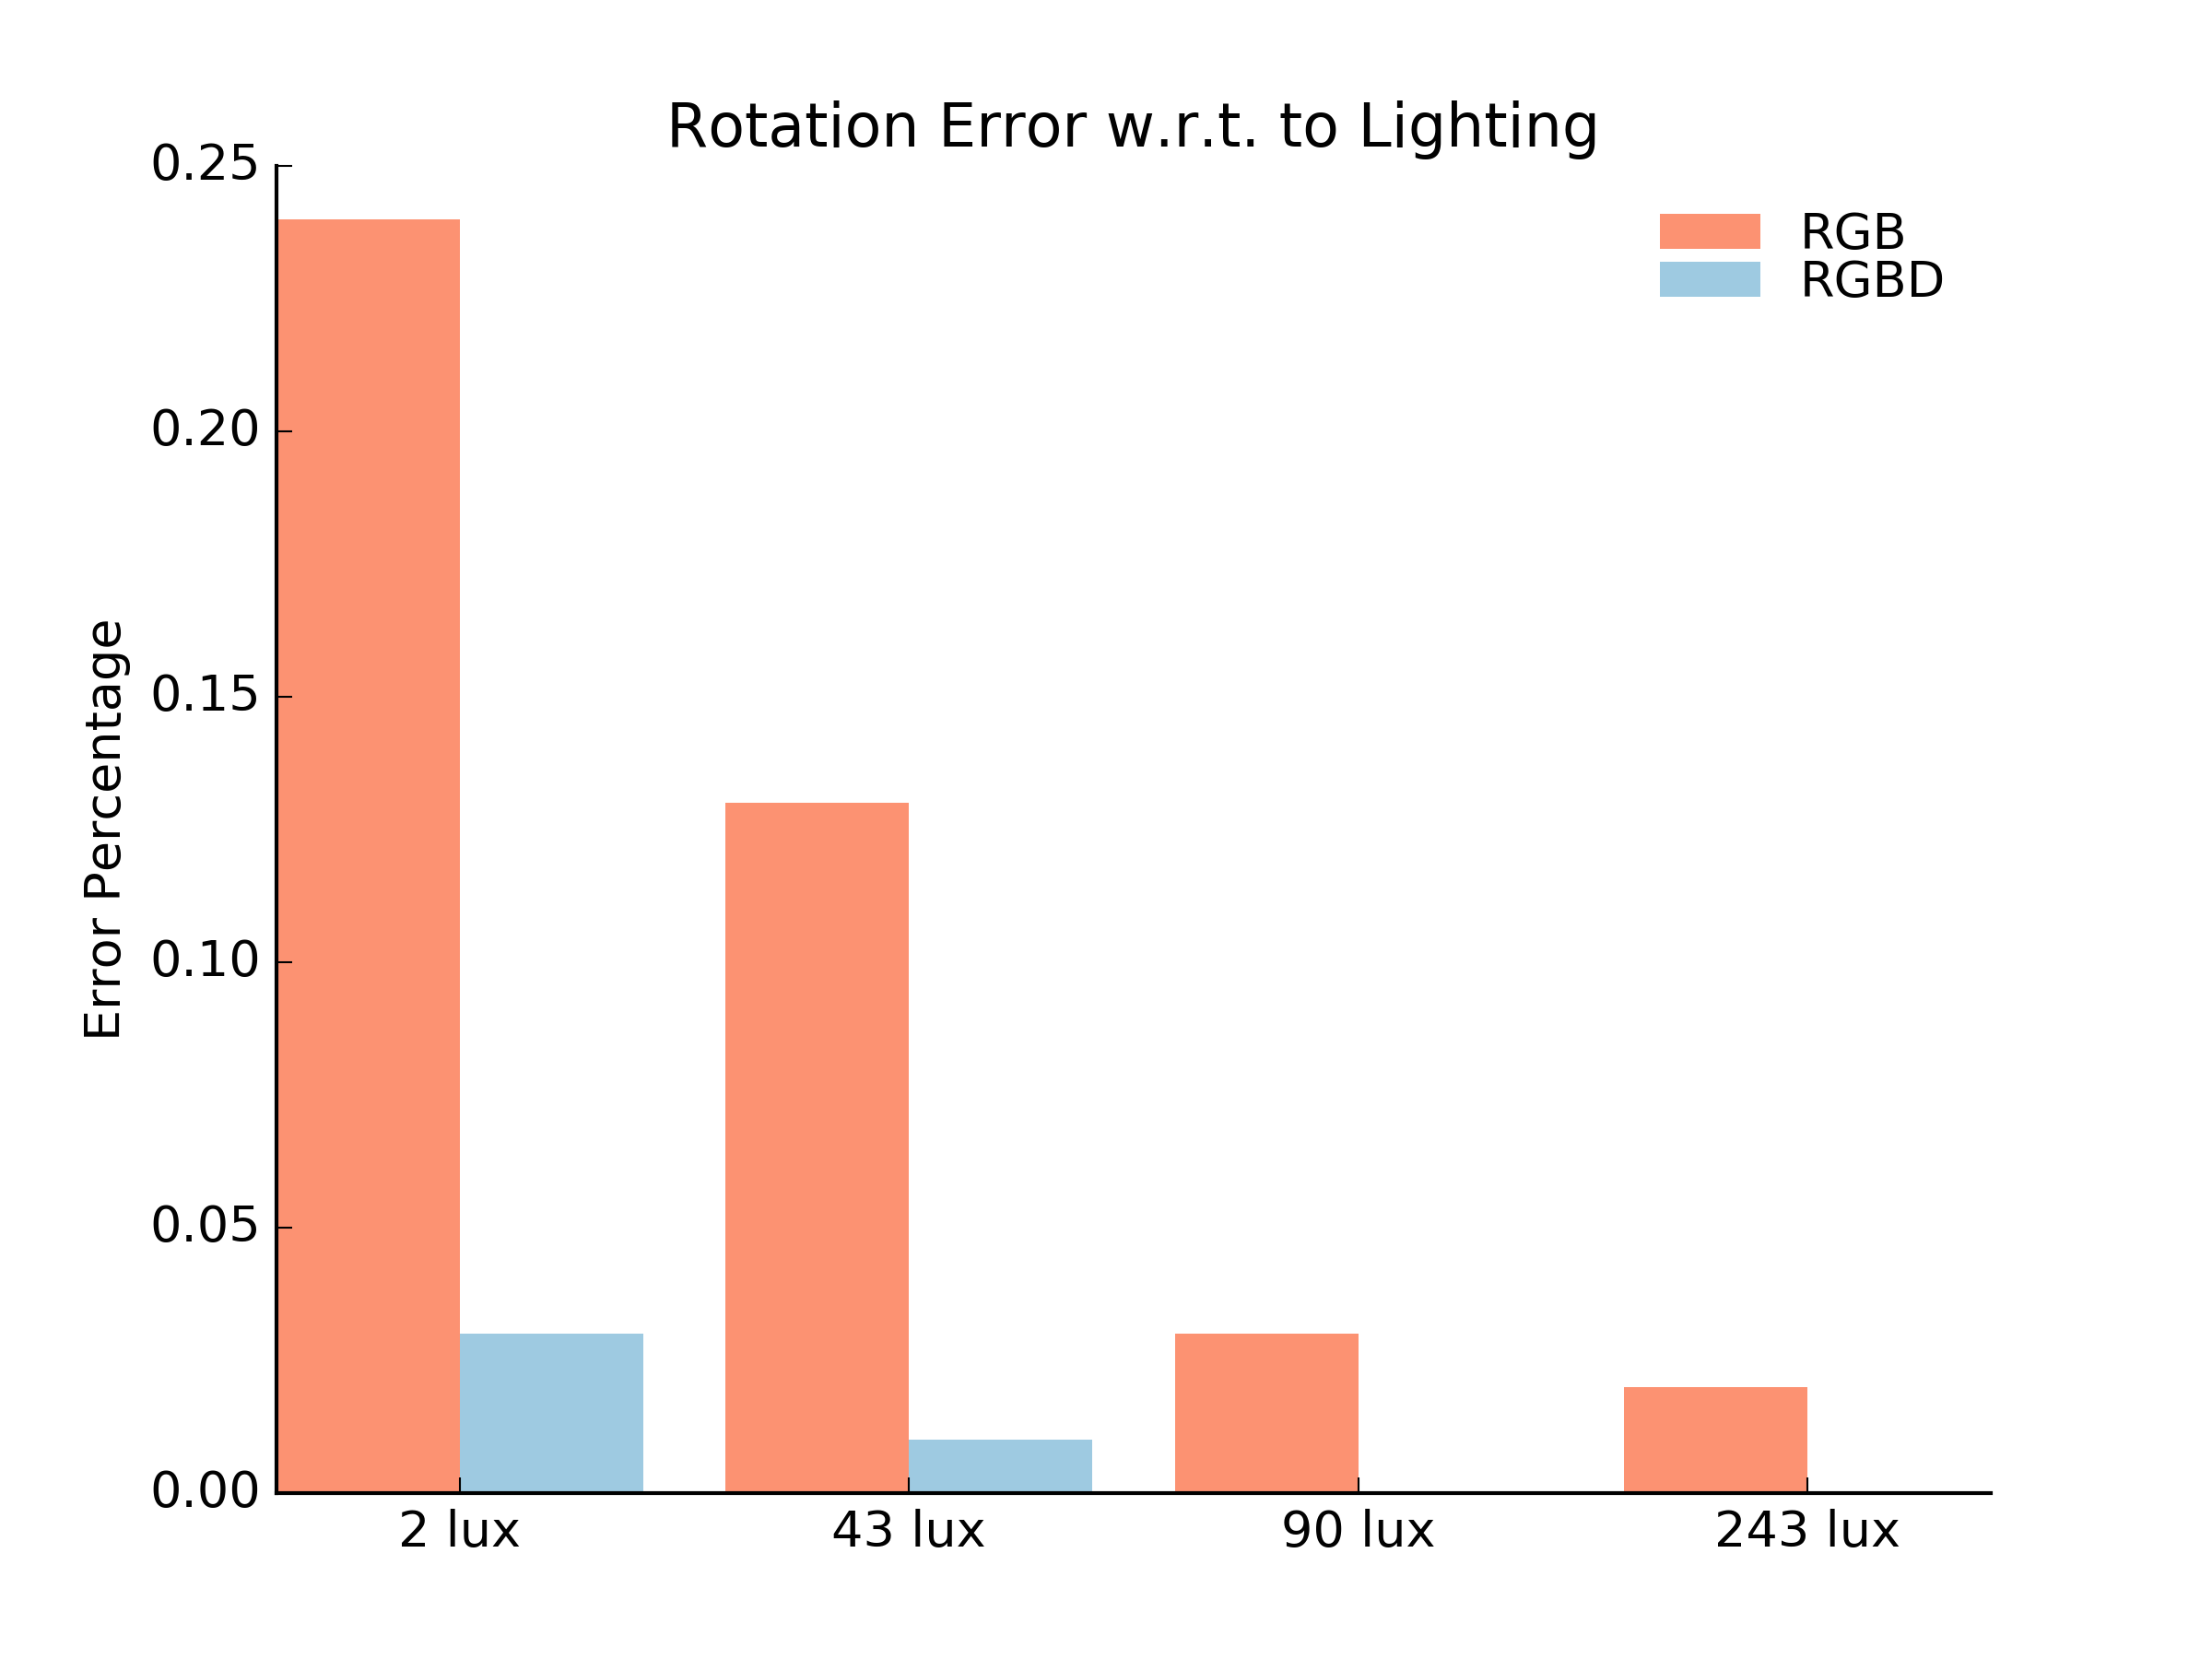
\includegraphics[width=\columnwidth]{figs/lighting_fig1}
\caption{Illumination vs Error Percentage. Data are captured at $65$ cm away from the camera at a $40$ degree angle.}
\label{fig:lighting_result}
\end{figure}

\subsection{Lighting}

From our past observations, poor lighting condition is the most significant contributing factor to noise and it results in low localization accuracy. The Kinect V2 sensor used in our experiments dynamically adjust the exposure time under low lighting conditions. When pictures are taken below or near the adjustable range of the sensor, they contain very noticeable noise as shown in Figure \ref{fig:illumination_tag}.

We also tested the algorithm under harsh lighting conditions in a real world setting. The data were captured under 4 different lighting conditions: 20 lux (dark), 43 (lux) dim, and (90 lux) normal, 243 lux (bright). We recorded a static scene over 5 seconds and randomly sampled 100 frames to run the test.  As results shown in Figure \ref{fig:lighting_result}, the localization accuracy significantly improves with better illumination. At the lowest illumination, nearly $25\%$ of the poses were unacceptable (more than $20$ degrees off) at the particular viewing angle. By using depth sensor which is unaffected by poor source radiance, there are only ~$3\%$ of unacceptable poses.

\subsection{Benchmark Against ar\_track\_alvar}

\begin{figure}
\centering
\subfloat[Rotation Error]{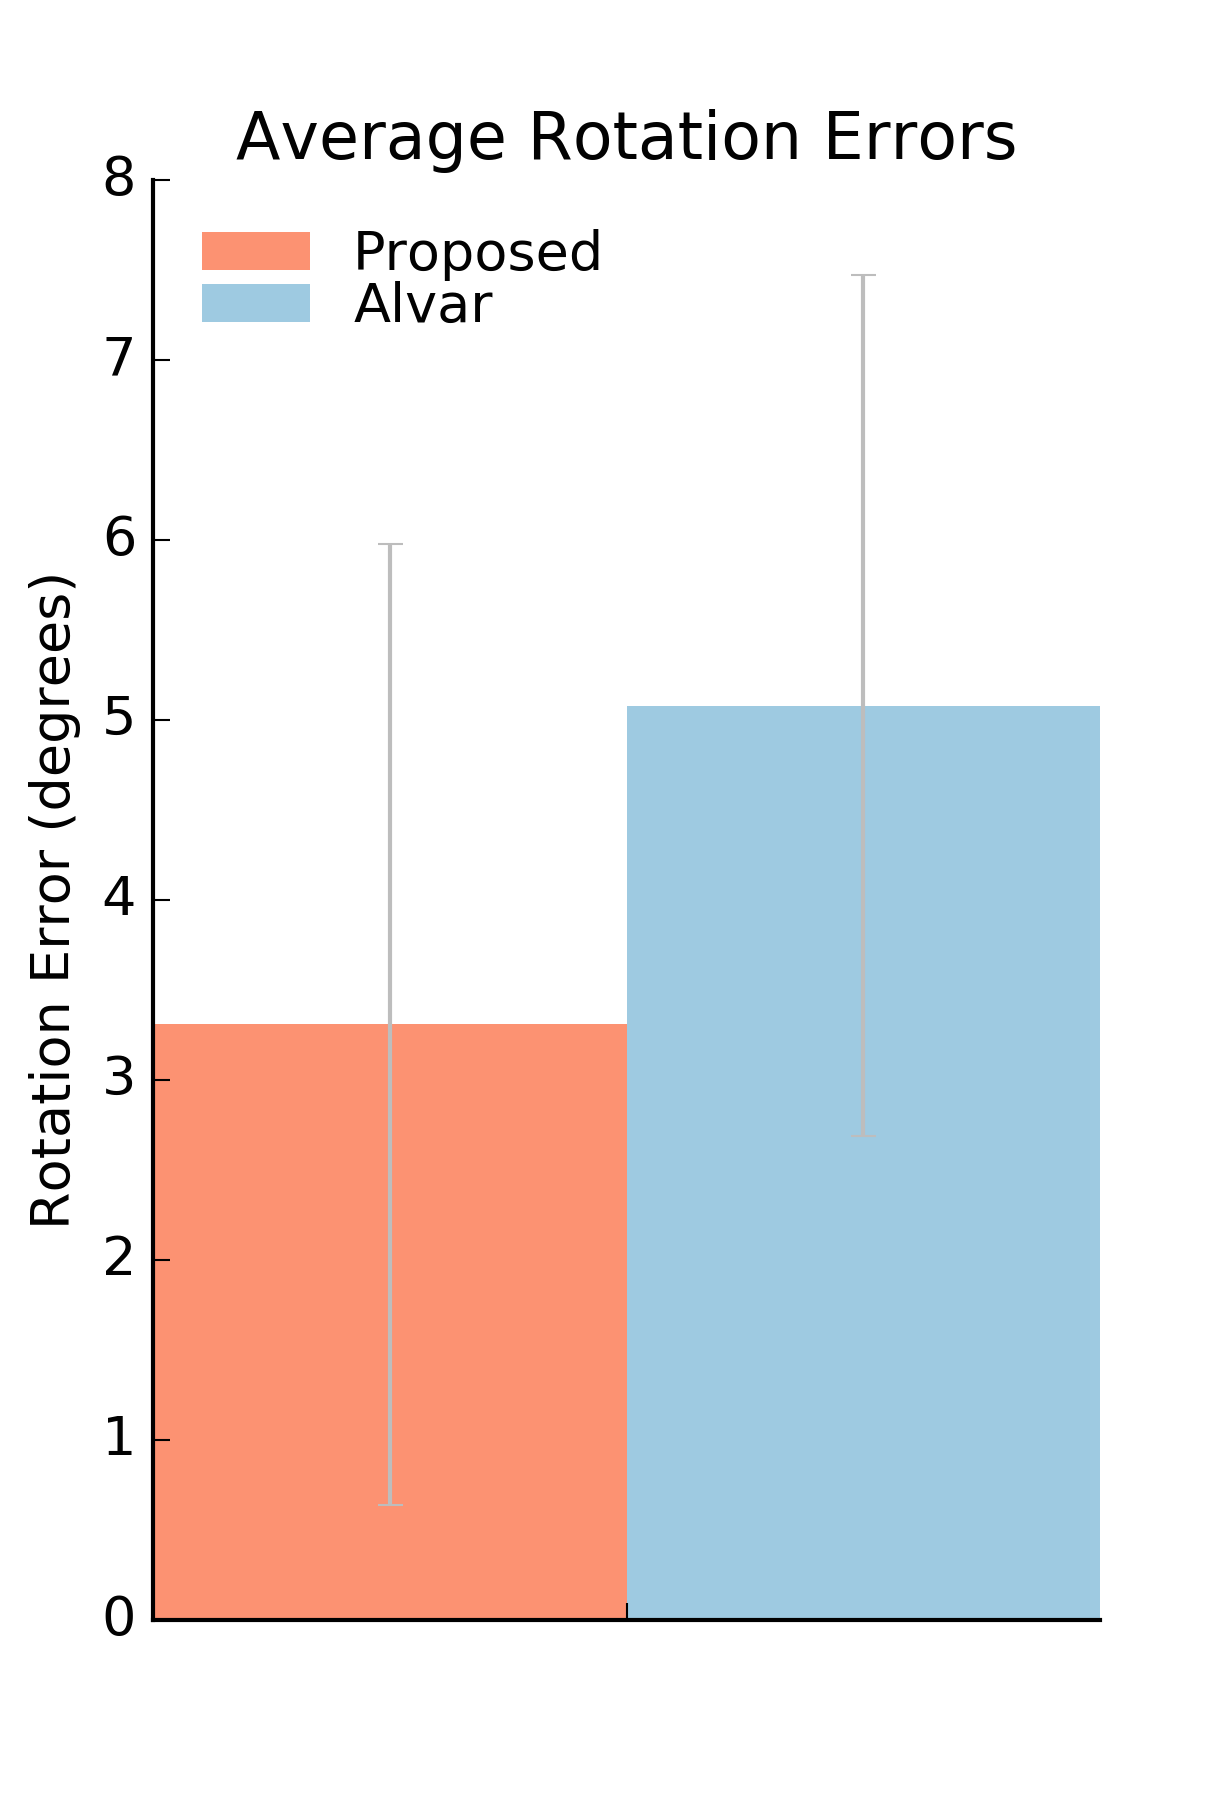
\includegraphics[width=120px, height=180px]{figs/alvar_rot}}
\subfloat[Translation Error]{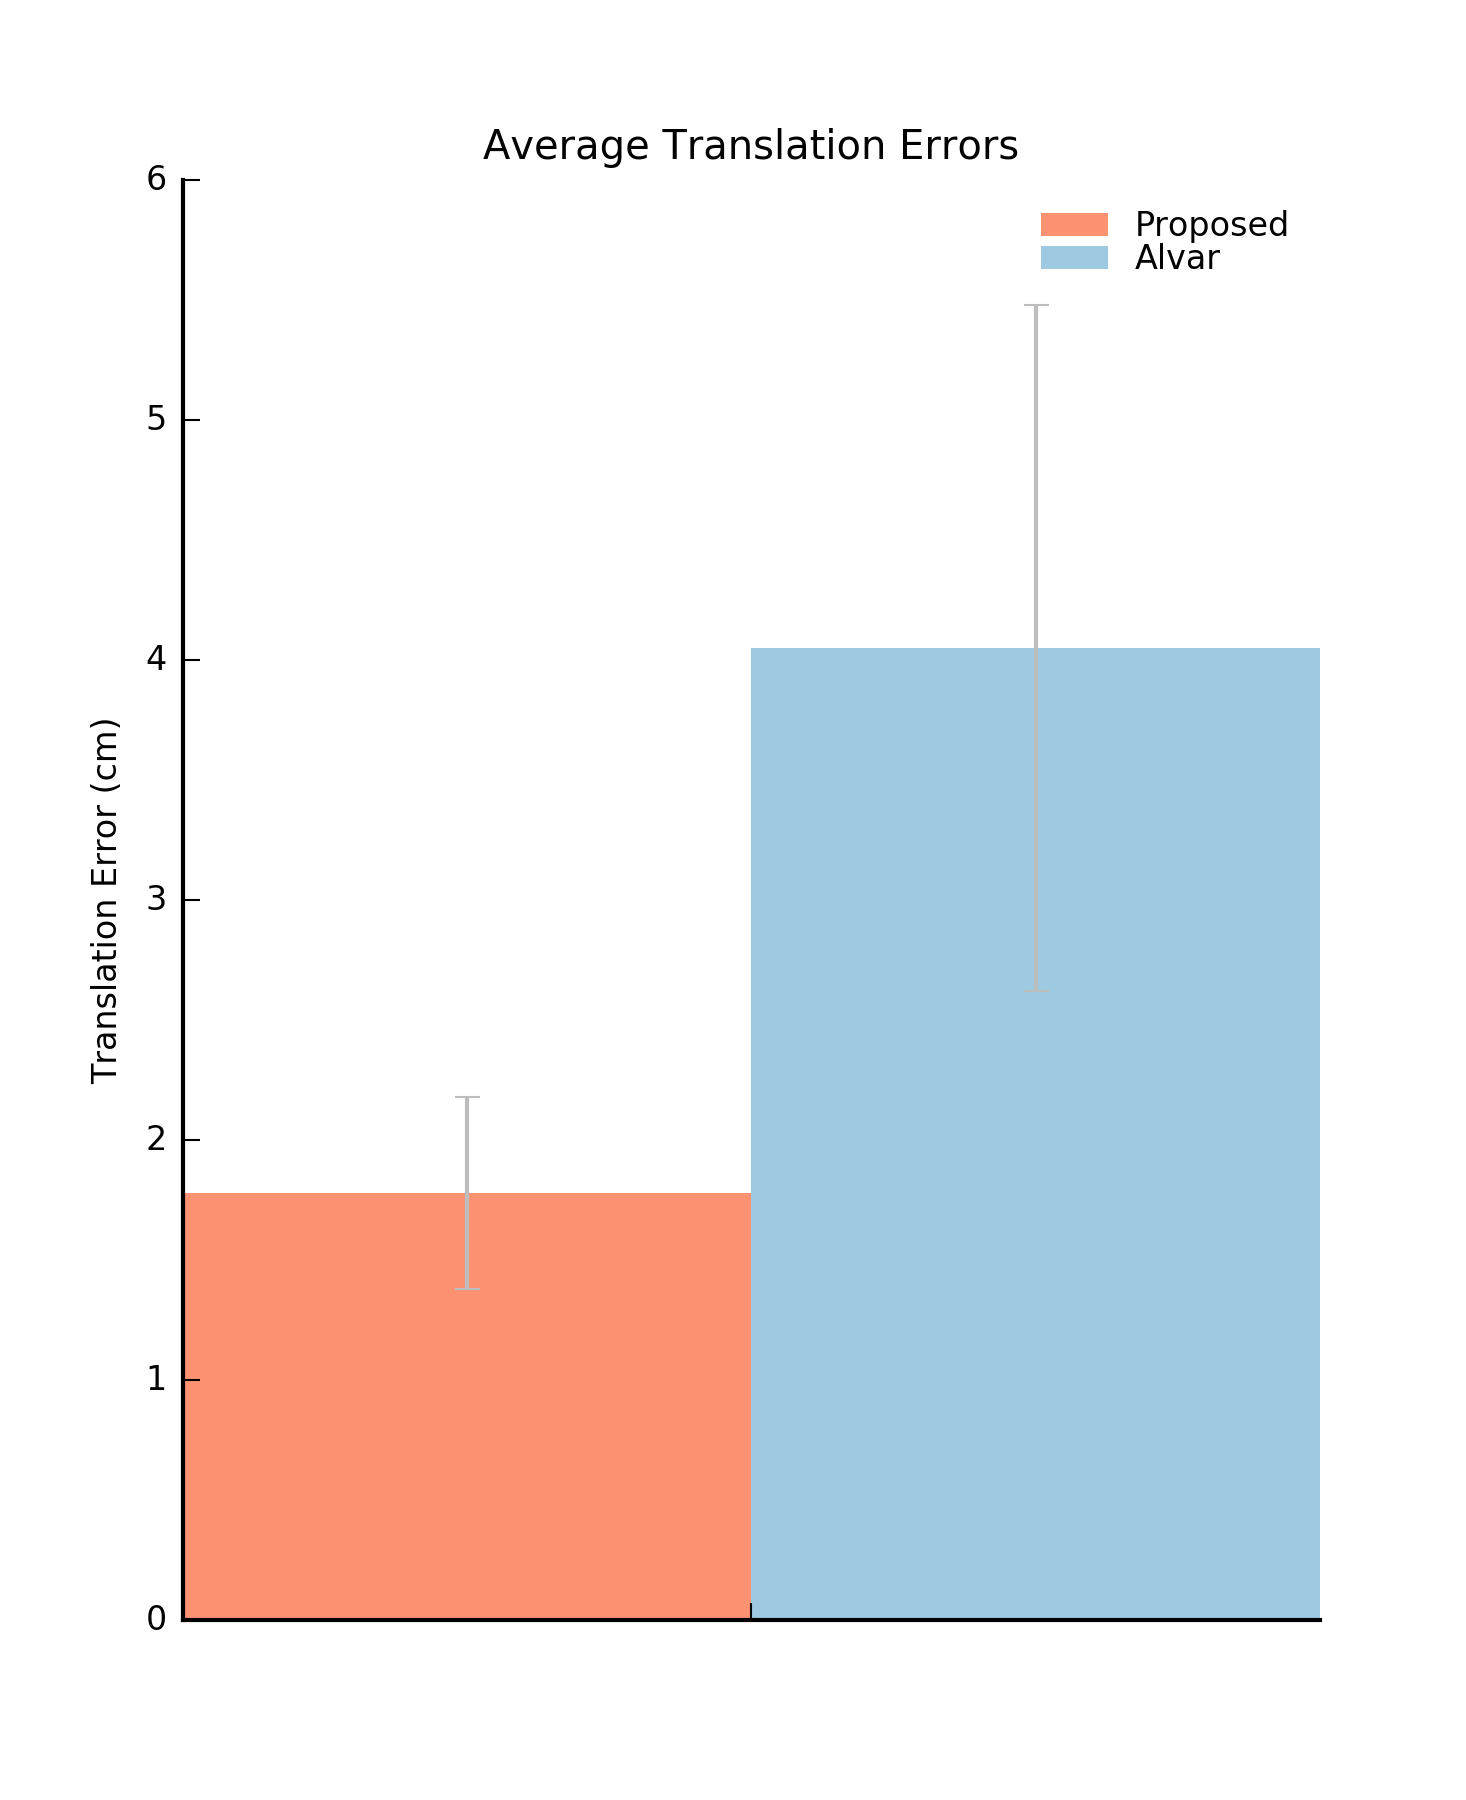
\includegraphics[width=120px, height=180px]{figs/alvar_trans}}
\caption{Average pose errors compared with \textit{ar\_track\_alvar} package.}
\label{fig:alvartrack}
\end{figure}

\textit{ar\_track\_alvar} is a ROS wrapper package for Alvar \citep{alvartrack}, an open source AR tag tracking library. The package is designed for AR tag detection and pose estimation for robots similar to Apriltags. In particular, it implements a module where depth sensor is integrated to improve the pose estimation. The package use the detected corner points to extract a patch of point clouds containing the tag. Then it proceed to fit a plane of the point cloud data and find its centroid using PCL. The pose of the tag is computed by aligning the centroid with the center of the tag.   

We implemented a similar module for the Apriltag and compared the pose accuracy between our proposed method and the module using all the collected data. The results are shown in Figure \ref{fig:alvartrack}. The two algorithms performed similarly in rotation error, but the proposed method was on average $2$ cm better with the position component. The spread of error is also much smaller for the position component indicating that our purposed method is more consistent.

\subsection{Computation Time}
We briefly tested the computation time of the new algorithm. With our current implementation in Python, the additional computation time for sensor fusing process is ~$11$ ms. Therefore the entire detection pipeline can process a $960$ x $540$ image within $35$ ms. All tag detectors and the fusing process were running in a single-threaded mode of an Intel core. Since our sensory updates at roughly $35Hz$, the entire pipeline can process the tags and estimate the pose in near real time. There is no significant time increase on a higher resolution image for the fusing process because our algorithm does not need to process the entire image.

% !TEX root = ../main.tex
\section{Conclusion}
\label{sec:conclusion}
% An important extension of the purposed method is to formally define the perceptual uncertainty produced by the pose estimation algorithm. For example, if the detector knows the pose estimated have large margins of error, it is useful to have some notion of uncertainty around the estimated pose. This is especially helpful inputs to any motion planing algorithms that takes uncertainty into consideration.

In this paper, we did a in depth analysis of the localization problem with Apriltags. We proposed a novel algorithm of using RGBD sensors to accurately compute the pose of Apriltags robust to noise. It is particularly suitable for robotic applications which requires precise poses such as manipulation, SLAM, and others. Furthermore, this technique can be easily generalized to other types of planar fiducial tags. Our implementation is fully open sourced and available at:

	http://somegithublink.com

\footnotesize{
\bibliographystyle{abbrv}
\bibliography{bib/references}
}
\end{document}

